% pdflatex paper.tex
% biber paper.bcf
% pdflate paper.tex (x2)

\documentclass[twoside]{article}

\usepackage[sc]{mathpazo}
\usepackage[utf8]{inputenc}
\usepackage[english,italian]{babel}
\linespread{1.05} % Line spacing - Palatino needs more space between lines
\usepackage{microtype} % Slightly tweak font spacing for aesthetics

\usepackage{graphicx}
\usepackage[hmarginratio=1:1,top=32mm,columnsep=20pt, margin=2.5cm]{geometry} % Document margins
%\usepackage{multicol} % Used for the two-column layout of the document
\usepackage[hang, small,labelfont=bf,up,textfont=it,up]{caption} % Custom captions under/above floats in tables or figures
\usepackage{booktabs} % Horizontal rules in tables
\usepackage{float} % Required for tables and figures in the multi-column environment - they need to be placed in specific locations with the [H] (e.g. \begin{table}[H])
\usepackage{hyperref} % For hyperlinks in the PDF
\usepackage{listings}

\usepackage{lettrine} % The lettrine is the first enlarged letter at the beginning of the text
\usepackage{paralist} % Used for the compactitem environment which makes bullet points with less space between them

\usepackage{geometry} % Impostazioni margini
\geometry{a4paper,top=3cm,bottom=3cm,left=1.30cm,right=1.30cm,%
    heightrounded,bindingoffset=5mm}
    
\usepackage{textcomp} % Impostazioni codici
\usepackage[T1]{fontenc}
\lstset{
  basicstyle=\ttfamily,
  columns=flexible,
  upquote,
}

\usepackage{abstract} % Allows abstract customization
\renewcommand{\abstractnamefont}{\normalfont\bfseries} % Set the "Abstract" text to bold
\renewcommand{\abstracttextfont}{\normalfont\small\itshape} % Set the abstract itself to small italic text

\usepackage{titlesec} % Allows customization of titles
\renewcommand\thesection{\Roman{section}} % Roman numerals for the sections
\renewcommand\thesubsection{\Roman{subsection}} % Roman numerals for subsections
\titleformat{\section}[block]{\large\scshape\centering}{\thesection.}{1em}{} % Change the look of the section titles
\titleformat{\subsection}[block]{\large}{\thesubsection.}{1em}{} % Change the look of the section titles
%\usepackage{fancyhdr} % Headers and footers
%\pagestyle{fancy} % All pages have headers and footers
%\fancyhead{} % Blank out the default header
%\fancyfoot{} % Blank out the default footer
%\fancyhead[C]{$\bullet$ Gennaio 2016 $\bullet$} % Custom header text
%\fancyfoot[RO,LE]{\thepage} % Custom footer text

\usepackage{amsmath}
\usepackage{txfonts}
\usepackage{enumitem}

\usepackage{subcaption}

\usepackage{biblatex}
\bibliography{bibliography}

\setlength\parindent{0pt} % Nessuna rientranza ad inizio paragrafo
\setlength\parskip{10pt} % Spaziatura tra paragrafi

%----------------------------------------------------------------------------------------
% IMPOSTAZIONI DI SILLABAZIONE
%----------------------------------------------------------------------------------------

\hyphenation{dynamo baseball cluster consistency COPS replication availability partition-tolerance Communications SIGOPS annual preserving performance}
% Inserire le parole che non devono essere sillabate e spezzate da tex

%----------------------------------------------------------------------------------------
%	CUSTOM MACRO
%----------------------------------------------------------------------------------------

\newcommand{\vclock}{\mathrm{VC}} % VC

%----------------------------------------------------------------------------------------
%	TITLE SECTION
%----------------------------------------------------------------------------------------

\title{\vspace{-15mm}\fontsize{24pt}{10pt}\selectfont\textbf{Configurazione di application server in ambiente di cloud computing}} % Article title

\author{
\large
\textsc{Bartolomeo Lombardi, Amerigo Mancino, Andrea Segalini}\\[2mm] % Your name
\normalsize Università degli Studi di Bologna % Your institution
\vspace{5mm} \\
\normalsize \href{mailto:bartolomeo.lombardi@studio.unibo.it}{bartolomeo.lombardi@studio.unibo.it}\\
\normalsize \href{mailto:amerigo.mancino@studio.unibo.it}{amerigo.mancino@studio.unibo.it}\\
\normalsize \href{mailto:andrea.segalini@studio.unibo.it}{andrea.segalini@studio.unibo.it}
\vspace{-5mm}
}
\date{Anno Accademico 2015-16}

%----------------------------------------------------------------------------------------

\begin{document}
\maketitle 
%\thispagestyle{fancy} % All pages have headers and footers

%----------------------------------------------------------------------------------------
%	ABSTRACT
%----------------------------------------------------------------------------------------

\begin{abstract}
\noindent
OpenNebula è un toolkit che offre una soluzione semplice ma flessibile per la costruzione e la gestione
di soluzioni cloud e di centri di elaborazione dati distribuiti eterogenei.
In questa breve relazione ci proponiamo di illustrare, passo dopo passo, il lavoro fatto, consistente
nell'installazione e nella configurazione dei software OpenNebula e JBoss, oltre che nella scrittura
di un piccolo programma JBoss volto a dimostrare le proprietà di tolleranza ai guasti e migrazione.
Verranno poi discusse le varie problematiche incontrate e saranno mostrati i metodi che hanno portato
alla loro risoluzione.
\end{abstract}

%----------------------------------------------------------------------------------------

\vspace{15mm} % Spaziatura tra abstract e corpo articolo %% backup {20mm}

%----------------------------------------------------------------------------------------
%	ARTICLE CONTENTS
%----------------------------------------------------------------------------------------



\section{Introduzione: tecnologie utilizzate}
Per creare un sistema di cloud e poter dimostrare, di conseguenza, le proprietà di migrazione e
tolleranza ai guasti volute ci si è serviti di due tecnologie principali:
\begin{itemize}
	\item OpenNebula \cite{bib:opennebula2} \\
		  Progetto open source per sistemi GNU/Linux supportato da una vasta community, in grado di
		  creare e gestire strutture cloud e data center virtualizzati. Differentemente da altre soluzioni,
		  OpenNebula si pone come un sistema aperto, flessibile e personalizzabile in base alle esigenze
		  oltre che robusto, in grado di fornire anche funzionalità innovative per cloud privati e ibridi.
		  Inoltre permette la realizzazione di cloud Iaas (Infrastructure as a Service), permettendo integrità
		  anche nel caso di macchine eterogenee dal punto di vista hardware e software. Come unico requisito
		  richiede un hardware con supporto per la virtualizzazione.
	\item JBoss \cite{bib:jboss2} \\
		  WildFly, precedentemente noto come JBoss, è un application server open source che implementa
		  le specifiche Java EE. Fra le numerose componenti di cui è costituito il prodotto, sottolineiamo
		  le funzionalità di clustering (che funge da load balancer), di failover (invio di componenti di
		  un sistema ad una seconda componente quando la prima presenta qualche problema), di distributed
		  caching, oltre che di implementazione distribuita. Tutte queste caratteristiche la rendono una
		  ottima piattaforma di sviluppo.
\end{itemize}

\section{Configurazione di OpenNebula}
L'installazione di OpenNebula avviene in maniera differente a seconda del ruolo giocato dal componente.
Si distingue il Front-end, ossia colui che esegue OpenNebula, instanzia le macchine virtuali sugli altri
membri e gestisce di fatto l'intera rete cloud, e i Worker, i quali eseguono invece la macchine virtuali
instanziate dal Front-end.

Per stabilire la comunicazione fra Front-end e Worker è stato usato un router, creando una rete ad hoc 
e sono stati impostati gli indirizzi IP staticamente.
Il Front-end è stato installato su sistema Ubuntu 14.04 ed è stata seguita
la procedura di installazione illustrata nella documentazione ufficiale di OpenNebula \cite{bib:opennebula},
mentre sui Worker è stato montato Ubuntu 15.10.
La configurazione della rete che abbiamo realizzato è mostrata in Figura \ref{fig:4}.
I comandi preceduti da \# sono da considerare eseguiti da utente root, il cui passaggio è consentito
mediante il comando:
\begin{lstlisting}[frame=trBL]
sudo su
\end{lstlisting}
mentre quelli preceduti da \$ vanno intesi eseguiti da oneadmin, creato durante l'installazione del
repository.

\begin{figure}[!tbp]
\centering
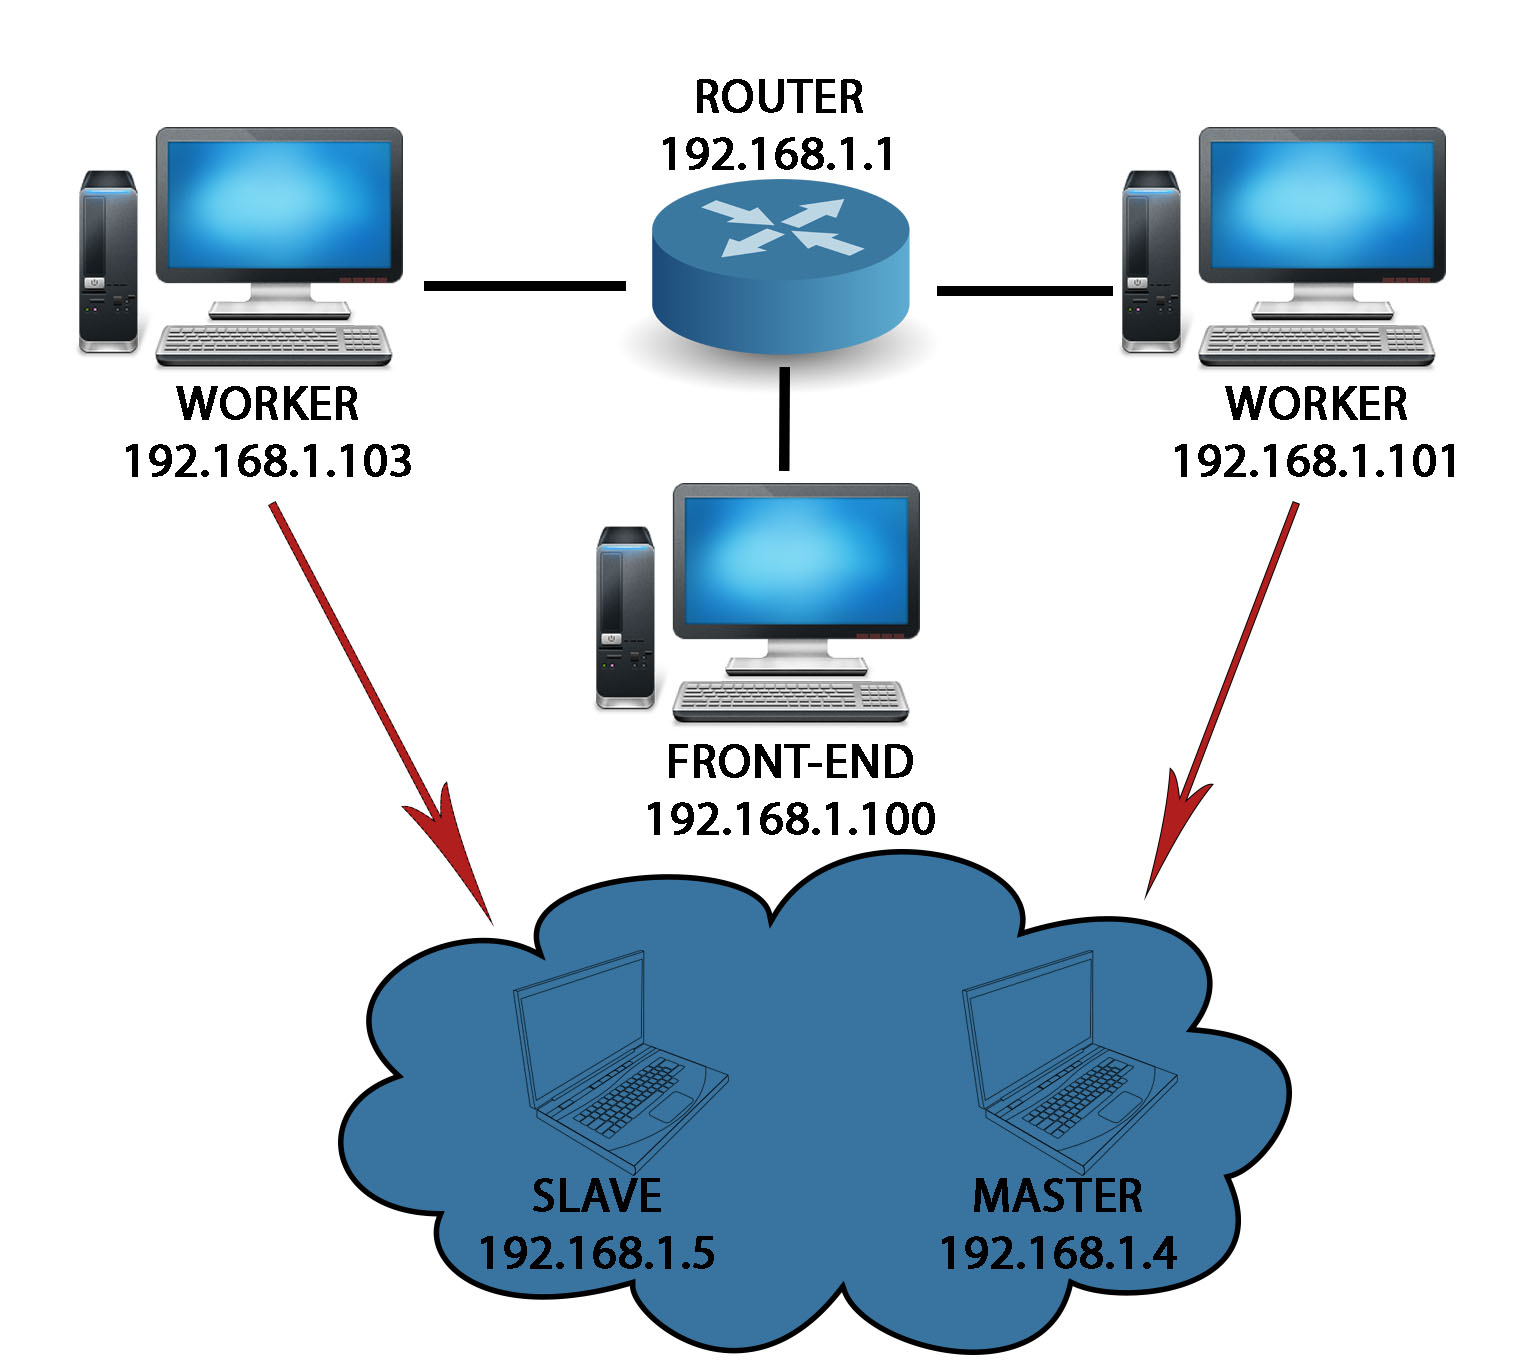
\includegraphics[width=13cm]{immagine4.jpg}
\caption{COnfigurazione della nostra rete}\label{fig:4}
\end{figure}

\section{Configurazione di OpenNebula su Front-end}
In primo luogo abbiamo verificato il supporto alla virtualizzazione eseguendo il comando:
\begin{lstlisting}[frame=trBL]
grep -E 'svm|vmx' /proc/cpuinfo
\end{lstlisting}

Successivamente ci siamo curati di aggiungere il repository di OpenNebula:
\begin{lstlisting}[frame=trBL]
# wget -q -O- http://downloads.opennebula.org/repo/Ubuntu/repo.key | apt-key add -
# echo "deb http://downloads.opennebula.org/repo/4.12/Ubuntu/14.04/ stable 
  opennebula" \ > /etc/apt/sources.list.d/opennebula.list
\end{lstlisting}

E dell'installazione dei pacchetti necessari:
\begin{lstlisting}[frame=trBL]
# apt-get update
# apt-get install opennebula opennebula-sunstone nfs-kernel-server
\end{lstlisting}

A questo punto è stata configurata la Sunstone, ossia l'interfaccia grafica di OpenNebula:
abbiamo quindi modificato il file 
\texttt{/etc/one/sunstone-server.conf}, sostituendo la riga \texttt{:host:} \texttt{127.0.0.1}
con la riga \texttt{:host:} \texttt{0.0.0.0}, eseguendo poi il restart del servizio:
\begin{lstlisting}[frame=trBL]
# /etc/init.d/opennebula-sunstone restart
\end{lstlisting}

Dal momento che sono state usate delle macchine differenti nei nostri esperimenti, abbiamo optato
per la configurazione di un network file system distribuito: è stato necessario dunque esportare
\texttt{/var/lib/one/} dal Front-end ai nodi Worker, e aggiungere al file \texttt{/etc/exports}
del Front-end la riga:
\begin{lstlisting}[frame=trBL]
/var/lib/one/ *(rw,sync,no_subtree_check,root_squash)
\end{lstlisting}

Infine abbiamo fatto ripartire il servizio:
\begin{lstlisting}[frame=trBL]
# service nfs-kernel-server restart
\end{lstlisting}

OpenNebula ha bisogno poi di una chiave SSH senza password da ogni nodo (incluso il Front-end)
verso ogni altro nodo. Per impostarla, abbiamo eseguito i seguenti comandi:
\begin{lstlisting}[frame=trBL]
# su - oneadmin
$ cp ~/.ssh/id_rsa.pub ~/.ssh/authorized_key
\end{lstlisting}

E poi abbiamo aggiunto il seguente frammento al file \texttt{~/.ssh/config}:
\begin{lstlisting}[frame=trBL]
$ cat << EOT > ~/.ssh/config
Host *
    StrictHostKeyChecking no
    UserKnownHostsFile /dev/null
EOT
$ chmod 600 ~/.ssh/config
\end{lstlisting}

\section{Configurazione di OpenNebula su nodi Worker}
I Worker sono i nodi su cui vengono eseguite le macchine virtuali instanziate dal Front-end.
La configurazione è simile a quella appena illustrata per il Front-end: è stata scaricata la repo
e sono state installate tutte le dipendenze. Successivamente data la nostra scelta di utilizzare
il protocollo DHCP attraverso l'interfaccia \texttt{eth0} e l'uso di IP statici, come anticipato prima,
siamo andati a sostituire a sostituire il file \texttt{/etc/network/interfaces} con:
\newpage
\begin{lstlisting}[frame=trBL]
auto lo
iface lo inet loopback

auto br0
iface br0 inet static
        address 192.168.1.101
        network 192.168.1.0
        netmask 255.255.255.0
        broadcast 192.168.0.255
        gateway 192.168.0.1
        bridge_ports eth0
        bridge_fd 9
        bridge_hello 2
        bridge_maxage 12
        bridge_stp off
\end{lstlisting}
dove \texttt{192.168.1.101} rappresenta l'indirizzo di uno dei nostri Worker.
Per l'altro la procedura è assolutamente speculare.

Dopo aver fatto questi cambiamenti, abbiamo fatto ripartire il servizio:
\begin{lstlisting}[frame=trBL]
# /etc/init.d/networking restart
\end{lstlisting}

Poi abbiamo aggiunto al file \texttt{/etc/fstab} la riga:
\begin{lstlisting}[frame=trBL]
192.168.1.100:/var/lib/one/  /var/lib/one/  nfs   soft,intr,rsize=8192,wsize=8192,noauto
\end{lstlisting}

Dove \texttt{192.168.1.100} è l'indirizzo IP del Front-end. Infine è bastato eseguire:
\begin{lstlisting}[frame=trBL]
# mount /var/lib/one/
\end{lstlisting}

A questo punto abbiamo configurato Qemu, l'interfaccia che permette la simulazione delle macchine virtuali:
\begin{lstlisting}[frame=trBL]
# cat << EOT > /etc/libvirt/qemu.conf
user  = "oneadmin"
group = "oneadmin"
dynamic_ownership = 0
EOT
\end{lstlisting}

Per rendere effettivi i cambiamenti abbiamo fatto ripartire libvirt:
\begin{lstlisting}[frame=trBL]
# service libvirt-bin restart
\end{lstlisting}

Quando abbiamo provato a far comunicare il Front-end con un Worker attraverso il router
mediante un comando di ping la prima volta, inspiegabilmente abbiamo ottenuto un fallimento. Questo
era dovuto alla presenza di un firewall installato sul Front-end che è stato, dunque, opportunamente
disabilitato permettendo alle due macchine di vedersi e di comunicare.

\section{Preparazione dell'ambiente}
Come accennato in precedenza, ogni operazione in OpenNebula può essere fatta mediante
il terminale a riga di comando oppure utilizzando l'apposita interfaccia grafica Sunstone. Nelle nostre
prove abbiamo optato per la seconda opzione. Per accedere dunque alla Sunstone è sufficiente far puntare il
browser web (del Front-end chiaramente) all'indirizzo \texttt{http://localhost:9869}. La schermata
risultante non dovrebbe essere molto dissimile da quella mostrata in figura \ref{fig:3}.

\begin{figure}[!bp]
\centering
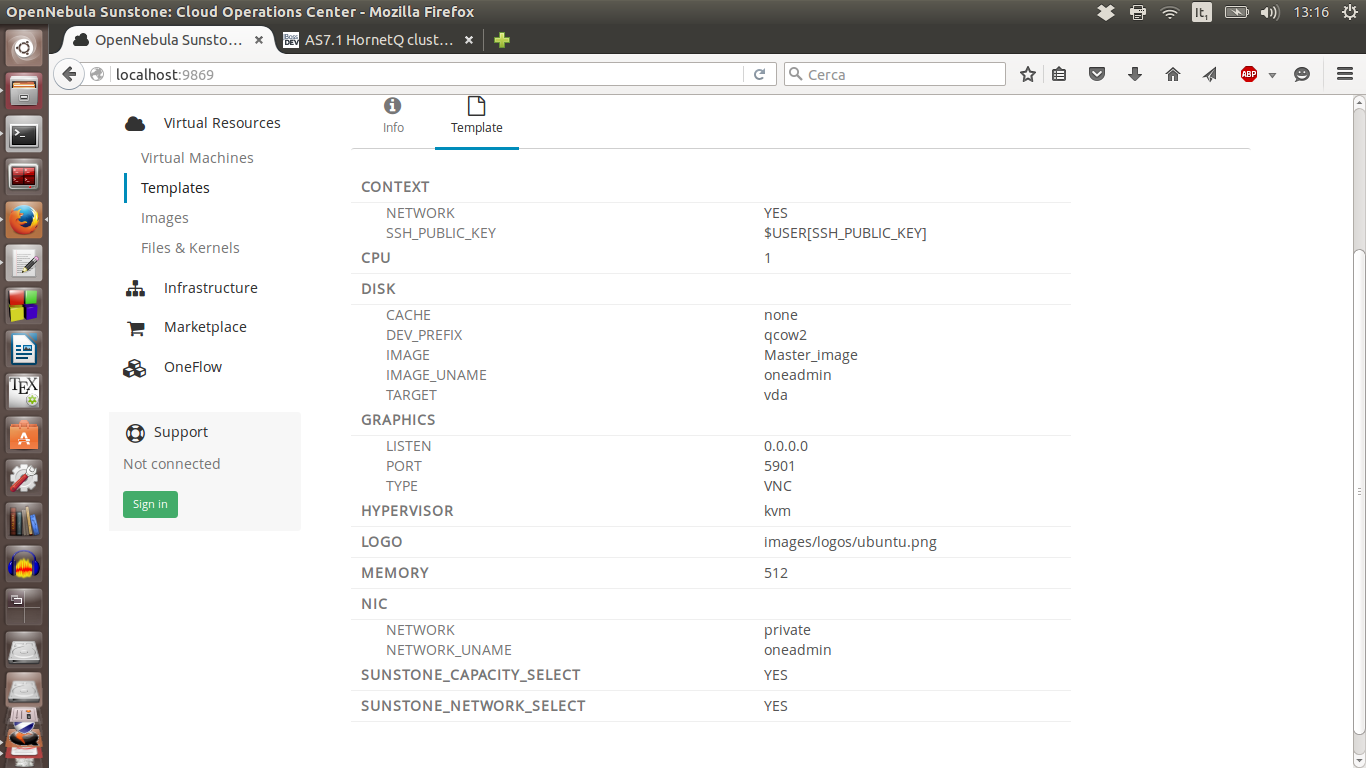
\includegraphics[width=13cm]{immagine3.png}
\caption{Sunstone di OpenNebula}\label{fig:3}
\end{figure}


A questo punto, è stato necessario preparare le immagini da inserire nel template della virtual machine.
Abbiamo quindi scaricato Ubuntu Server 14.04.3 LTS e dal Front-end abbiamo eseguito:
\begin{lstlisting}[frame=trBL]
$ qemu-img create -f qcow2 disk_image.img 5G
$ kvm -cpu host -smp 1 -m 1024 -cdrom nome_immagine.iso disk_image.img
\end{lstlisting}
Come si vede abbiamo usato kvm \cite{bib:kvm} per la virtualizzazione.

Usando kvm, quindi, il sistema è stato impreziosito con:
\begin{itemize}
	\item installazione SSH
\end{itemize}
\begin{lstlisting}[frame=trBL]
# apt-get install openssh-client openssh-server
\end{lstlisting}
\begin{itemize}
\item installazione di JBoss
\end{itemize}		  
\begin{lstlisting}[frame=trBL]
$ wget http://download.jboss.org/jbossas/7.1/jboss-as-7.1.1.Final/jboss-as-7.1.1.Final.tar.gz		  
\end{lstlisting}
Dopo aver fatto ciò, l'immagine è stata caricata su OpenNebula.

\section{Installazione di JBoss}
In questo paragrafo illustreremo l'installazione di JBoss \cite{bib:jboss}
che è stata eseguita sulla macchina virtuale che abbiamo precedentemente configurato. 
In primo luogo è stato necessario decomprimere l'archivio di JBoss.
Poi abbiamo spostato la cartella così ottenuta nella directory imposta come home di JBoss:
\begin{lstlisting}[frame=trBL]
tar xfvz jboss-as-7.1.1.Final.tar.gz
mv jboss-as-7.1.1.Final /opt/jboss
\end{lstlisting}

Per definire il cluster è stato necessario decidere quanti Slave lo compongono e
aggiungere i loro IP nel file \texttt{/etc/hosts}.

In seguito abbiamo creato un nuovo utente, eseguendo lo script \texttt{/opt/jboss/bin/add-user.sh}.
In questa dimostrazione è stato usato come nome utente \texttt{smuser} mentre come password abbiamo
banalmente impostato \texttt{password}.
Per configurare il Master affinché si possa comportare da domain controller si è modificato il file
\texttt{host.xml} specificando il suo indirizzo IP, cosicché gli Slave si possano connettere:
\begin{lstlisting}[frame=trBL]
<interfaces>
	<interface name="management">
		<inet-address value="${jboss.bind.address.management:192.168.1.4}"/>
	</interface>
	<interface name="public">
		<inet-address value="${jboss.bind.address:192.168.1.4}"/>
	</interface>
	<interface name="unsecured">
		<inet-address value="${jboss.bind.unsecured:192.168.1.4}" />
	</interface>
</interfaces>
\end{lstlisting}

Per configurare uno Slave, invece, abbiamo caricato una nuova immagine di Ubuntu su OpenNebula
e, dopo aver estratto JBoss e aver spostato la cartella risultante nella directory
impostata come sua home, abbiamo creato un nuovo utente JBoss, impostando come
user \texttt{slave1} e come password \texttt{123123}.
In seguito è stato modificato il file \texttt{host.xml}:

\begin{lstlisting}[frame=trBL]
<host name="slave" xmlns="urn:jboss:domain:1.2">
...
<domain-controller>
	<remote host="192.168.1.5" port="9999" security-realm="ManagementRealm"/>
</domain-controller>
...
<interfaces>
	<interface name="management">
		<inet-address value="${jboss.bind.address.management:192.168.1.5}"/>
	</interface>
	<interface name="public">
		<inet-address value="${jboss.bind.address:192.168.1.5}"/>
	</interface>
	<interface name="unsecured">
		<inet-address value="${jboss.bind.unsecured:192.168.1.5}" />
	</interface>
</interfaces>
...
\end{lstlisting}

Chiaramente è stato necessario gestire l'autenticazione: nel file \texttt{host.xml}
è stata cambiata la sezione \texttt{security-realms}, aggiungendo una nuova sezione \texttt{server-identities}
e modificando il valore dell'attributo value con quello in base64 della password dell'utente Slave,
ossia \texttt{123123}:
\newpage
\begin{lstlisting}[frame=trBL]
<security-realms>
	<security-realm name="ManagementRealm">
		<server-identities>
			<secret value="MTIzMTIz="/>
		</server-identities>
	<authentication>
		<properties path="mgmt-users.properties" relative-to="jboss.domain.config.dir"/>
	</authentication>
	</security-realm>
</security-realms>
\end{lstlisting}

Successivamente è stato installato nel Master il modulo \texttt{mod\char`_cluster} in modo tale da poterlo
usare da load balancer per il cluster. Dopo aver scaricato il pacchetto e averlo estratto,
si è spostata la cartella \texttt{httpd} in \texttt{opt/jboss/}:
\begin{lstlisting}[frame=trBL]
# wget
  http://downloads.jboss.org/mod_cluster//1.2.0.Final/
  mod_cluster-1.2.0.Final-linux2-x64-ssl.tar.gz
\end{lstlisting}
\begin{lstlisting}[frame=trBL]
tar xvf mod-cluster-1.2.0.Final-linux2-x64-ssl.tar.gz
cp -R mod-cluster-1.2.0-linux2-x86-ssl/httpd /opt/jboss/
\end{lstlisting}
\'{E} stato anche necessario modificare il file \texttt{/opt/jboss/httpd/httpd/conf/httpd.conf}:
\begin{lstlisting}[frame=trBL]
ServerName master

Listen 192.168.1.5:6666
<VirtualHost 192.168.1.5:6666>

<Directory />
	Order deny,allow
	Deny from all
	Allow from 192.168.1.
</Directory>

KeepAliveTimeout 60
MaxKeepAliveRequests 0

ManagerBalancerName other-server-group
AdvertiseFrequency 5

<Location /mod_cluster_manager>
	Order deny,allow
	Deny from all
	Allow from 192.168.1.
</Location>
</VirtualHost>
\end{lstlisting}
La direttiva di \texttt{Listener} permette di configurare l'indirizzo IP su cui il load balancer sarà
in attesa delle richieste mentre il tag \texttt{VirtualHost} permette invece di specificare l’indirizzo IP e
la porta di comunicazione tra il load balancer e gli application server.

\begin{figure}[!bp]
\centering
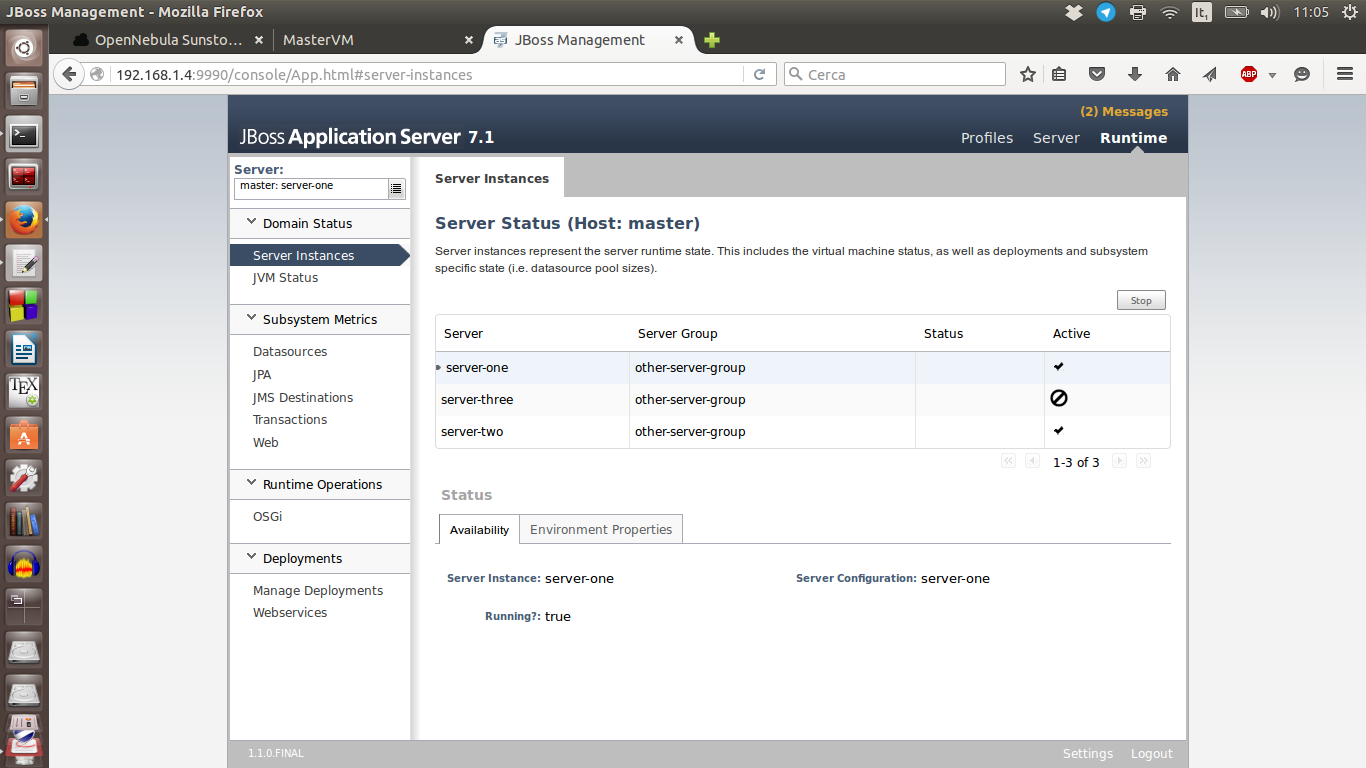
\includegraphics[width=13cm]{immagine1.png}
\caption{Interfaccia di JBoss}\label{fig:1}
\end{figure}

A questo punto non rimane che avviare httpd:
\begin{lstlisting}[frame=trBL]
/opt/jboss/httpd/sbin/apachectl start
\end{lstlisting}

Il servizio, nonostante si metta in moto correttamente, ci restituisce un warning indicante, a quanto pare,
che l'application engine non è in grado di determinare in maniera affidabile il nome di dominio del server;
in genere è dovuto a un problema di impostazione del file di configurazione di apache. Abbiamo ricontrollato
le modifiche fatte ai nostri file e ci sembrano corrette, ragion per cui abbiamo ignorato questo problema
proseguendo con l'avvio di JBoss. Questo warning è automaticamente sparito una volta completata
tutta la configurazione.

Per avviare JBoss è stato eseguito lo script:
\begin{lstlisting}[frame=trBL]
/opt/jboss/bin/domain.sh
\end{lstlisting}

A questo punto è stato possibile collegarsi all'interfaccia del servizio digitando l'indirizzo
\begin{lstlisting}[frame=trBL]
http://192.168.1.4:9990/console/App.html
\end{lstlisting}
nel browser web. Dopo aver quindi eseguito il login, la
schermata risultante non è molto dissimile a quella raffigurata in Figura \ref{fig:1}.
Abbiamo creato una applicazione JBoss che banalmente usa una variabile di sessione per registrare
e restituire, mediante operazioni di \texttt{get} e \texttt{put}, l'ora attuale. Ottenuto il war,
ne è stato fatto l'upload su JBoss e, subito dopo, il deploy. \'{E} stato quindi eseguito lo start di
tutti i server. Generalmente l'applicazione di default esegue su Server-Three, raggiungibile dalla
porta \texttt{8330}. Sono quindi stati fatti alcuni esperimenti di 
\texttt{http://192.168.1.4:8330/cluster-demo/put.jsp} e 
\texttt{http://192.168.1.4:8330/cluster-demo/get.jsp} che dimostrano il corretto funzionamento
dell'applicazione, come si può osservare in Figura \ref{fig:2}.

A questo punto abbiamo provato a fermare Server-Three: la sessione viene correttamente mantenuta
su Server-One, che diventa il server di default. Si può verificare questo collegandosi ad esso
mediante la porta \texttt{8080} (gli offset sono tutti specificati nel file \texttt{host.xml}).

\begin{figure}[!tbp]
\centering
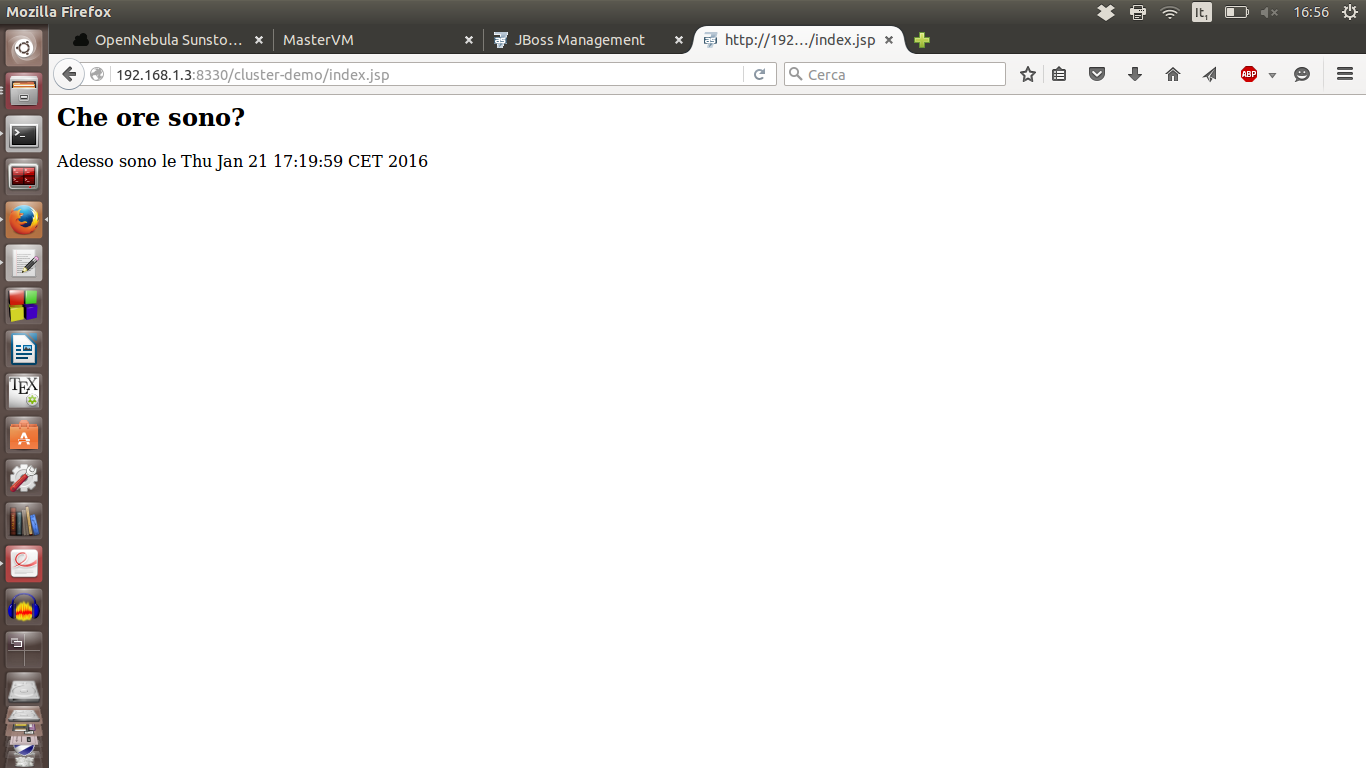
\includegraphics[width=13cm]{immagine2.png}
\caption{Esempio di esecuzione dell'applicazione JBoss}\label{fig:2}
\end{figure}

\section{Conclusioni e problematiche}
La configurazione dei software e dell'ambiente non è stata esente da problemi.
Le principali complicazioni riscontrate riguardano in primo luogo l'installazione di OpenNebula:
una volta scelto se installare il software come Worker, ad esempio, diventa particolarmente
ostico modificare la suddetta configurazione e quindi eventualmente tornare indietro per 
eseguire l'installazione come Front-end, a causa dei numerosi pacchetti e delle dipendenze che non vengono
automaticamente eliminate con il comando di \texttt{autoremove}. In seguito, si è avuta qualche difficoltà
anche nella configurazione di JBoss su virtual machine: in particolare, in seguito all'aggiunta
dell'utente \texttt{slave1}, \texttt{httpd} ha generato un errore
(causato probabilmente da alcuni nostri passaggi scorretti) che impediva il corretto
funzionamento dell'applicazione.
Questo problema è stato risolto unicamente ricaricando l'immagine di Ubuntu su OpenNebula e
ripetendo tutti i passaggi per garantire il corretto funzionamento di JBoss. \\
Il lavoro svolto ha quindi permesso, attraverso la configurazione dei software OpenNebula e JBoss, di
eseguire un'applicazione in ambiente di cloud computing e di dimostrare le proprietà di tolleranza ai guasti
e migrazione.


\printbibliography

\end{document}
